\begin{frame}{Analytic results: two transitions}
	\begin{tabular}{l l}
		\begin{minipage}{0.62\textwidth}
			\begin{equation*}
				\begin{cases}
					C_1 = \beta_1\epsilon e^{\beta_1\epsilon} \dfrac{\epsilon  + (\epsilon -\delta) e^{\beta_2\delta}}{T_1 \left( e^{\beta_1\epsilon} + 1 + e^{\beta_2\delta} \right)^2}\\
					\vspace{0pt}\\
					C_2 = \beta_2\delta e^{\beta_2\delta} \dfrac{\delta  + (\delta - \epsilon) e^{\beta_1\epsilon} }{T_2 \left( e^{\beta_1\epsilon} + 1 + e^{\beta_2\delta} \right)^2}
				\end{cases}
			\end{equation*}
			\begin{equation*}
				C_2 < 0 \Leftrightarrow \delta < \epsilon\dfrac{ e^{\beta_1\epsilon}}{1 + e^{\beta_1\epsilon} }
			\end{equation*}
			
		\end{minipage}
		&
		\begin{minipage}{0.38\textwidth}
			\vspace{-15pt}
			\begin{figure}
				\centering
				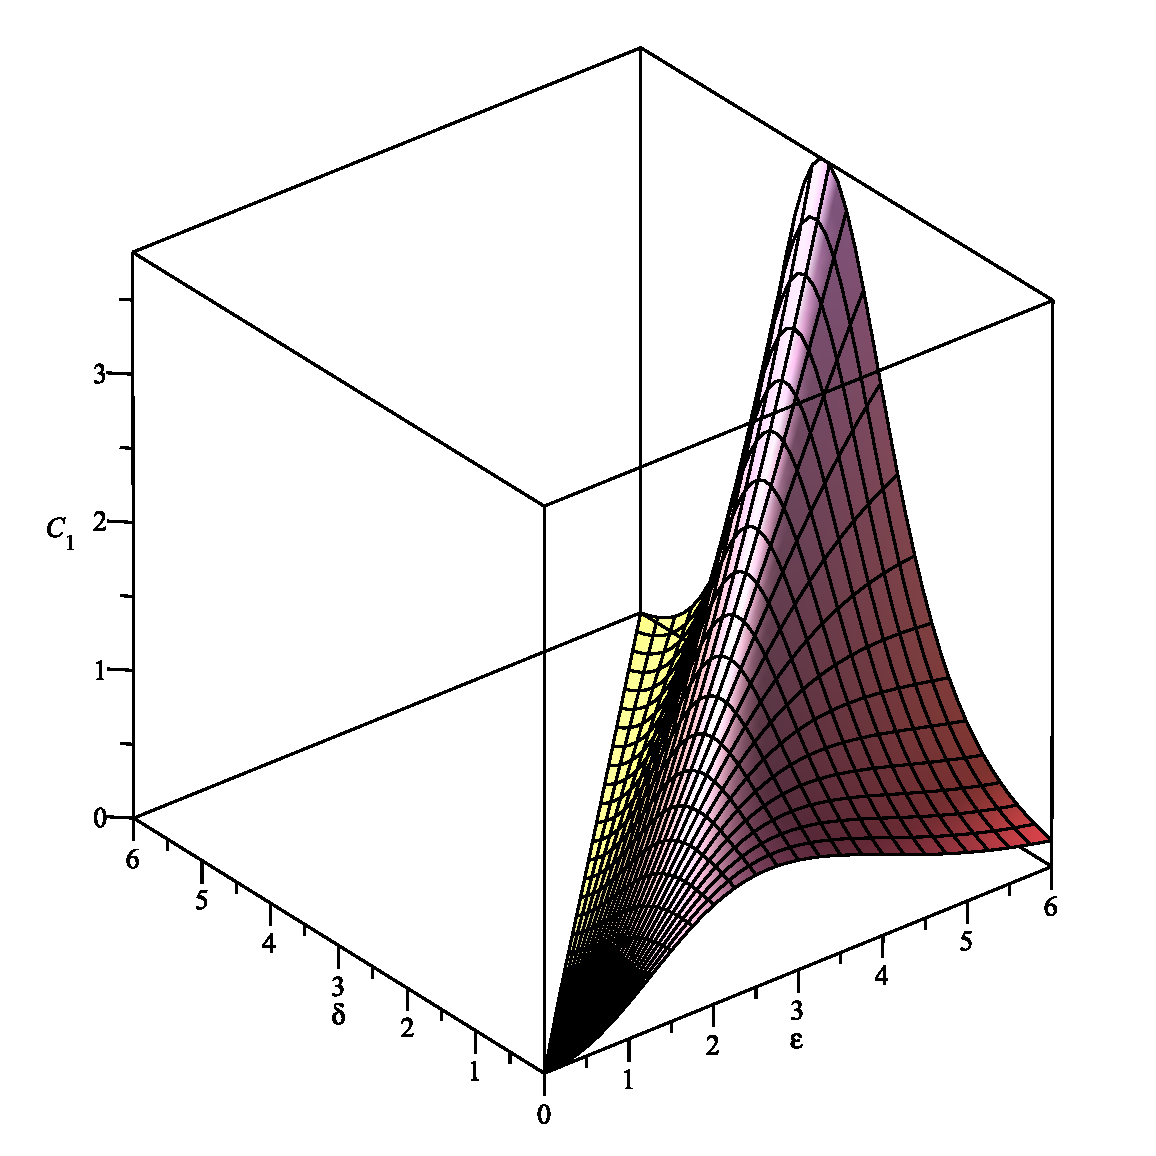
\includegraphics[height=0.44\textheight,keepaspectratio=true]{../src/plot/discreteSystems/C1InFunctionOfEpsilonAndDelta_1-eps-converted-to.pdf}
			\end{figure}
			\vspace{-25pt}
			\begin{figure}
				\centering
				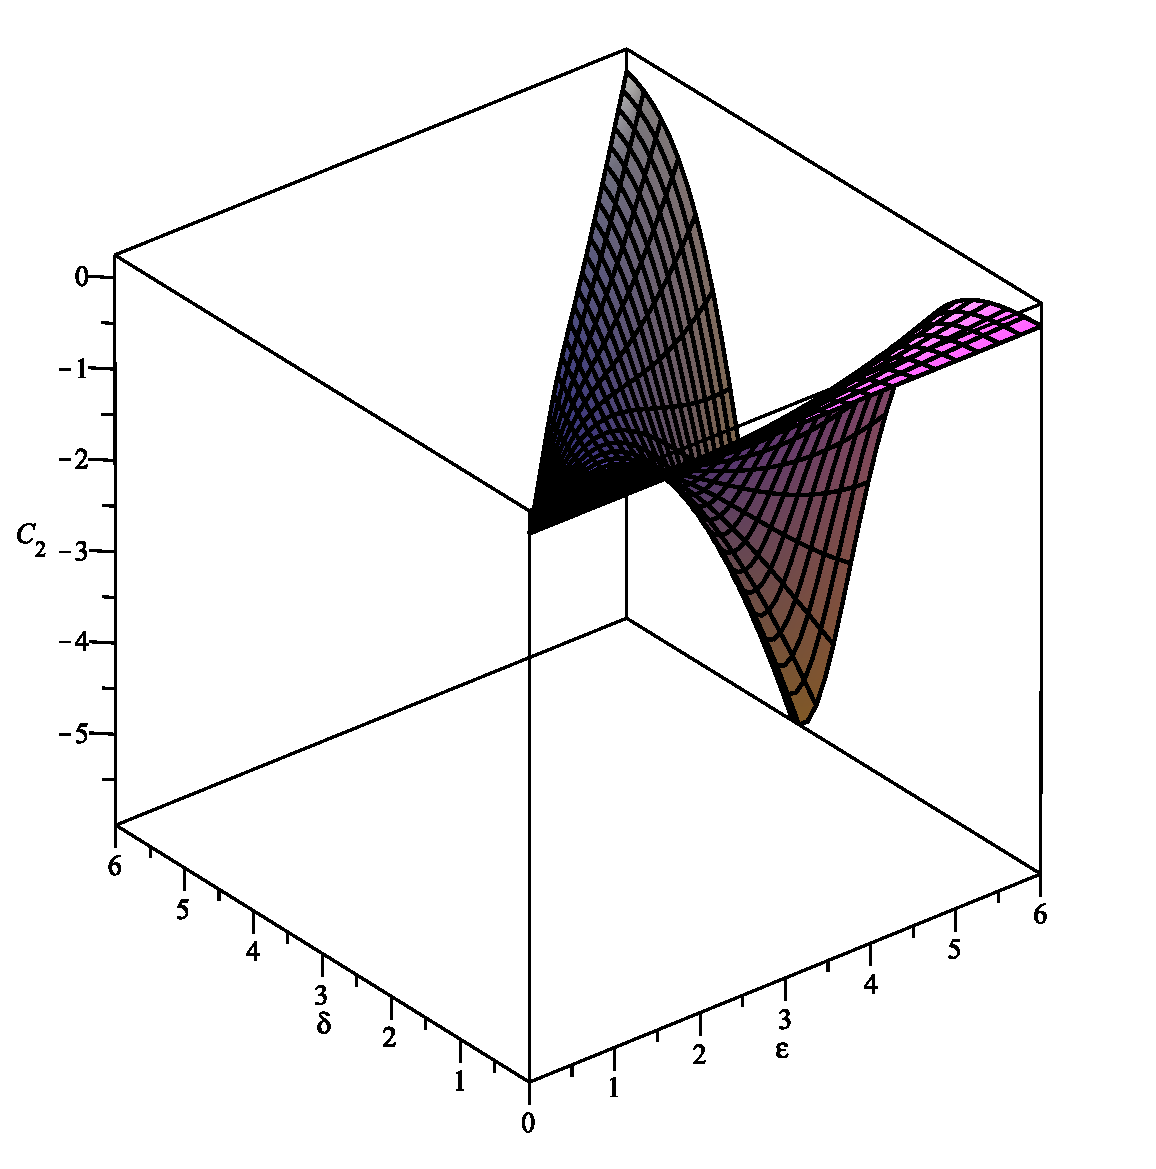
\includegraphics[height=0.44\textheight,keepaspectratio=true]{../src/plot/discreteSystems/C2InFunctionOfEpsilonAndDelta_1-eps-converted-to.pdf}
			\end{figure}
		\end{minipage}
	\end{tabular}
\end{frame}
%%%%%%%%%%%%%%%%%%%%%%%%%%%%%%%%%%%%%%%%


\begin{frame}{Analytic results: three transitions}

	\begin{tabular}{l l}
		\begin{minipage}{0.62\textwidth}
			\begin{equation*}
				\begin{cases}
				C_1 = \dfrac{\epsilon\beta_1 e^{-\beta_1\epsilon} (e^{-\beta_1\epsilon}\epsilon+\epsilon+\delta)}
				{T_1(e^{-\beta_1\epsilon} + 2)^3 (e^{-\beta_2\delta} + 2)}\\
				\vspace{0pt}\\
				C_2 = \dfrac{\delta\beta_2 e^{-\beta_2\delta} (e^{-\beta_2\delta}\delta+\epsilon+\delta)}
				{T_2(e^{-\beta_1\epsilon} + 2) (e^{-\beta_2\delta} + 2)^3}
				\end{cases}
			\end{equation*}
		\end{minipage}
		&
		\begin{minipage}{0.38\textwidth}
			\vspace{-15pt}
			\begin{figure}
				\centering
				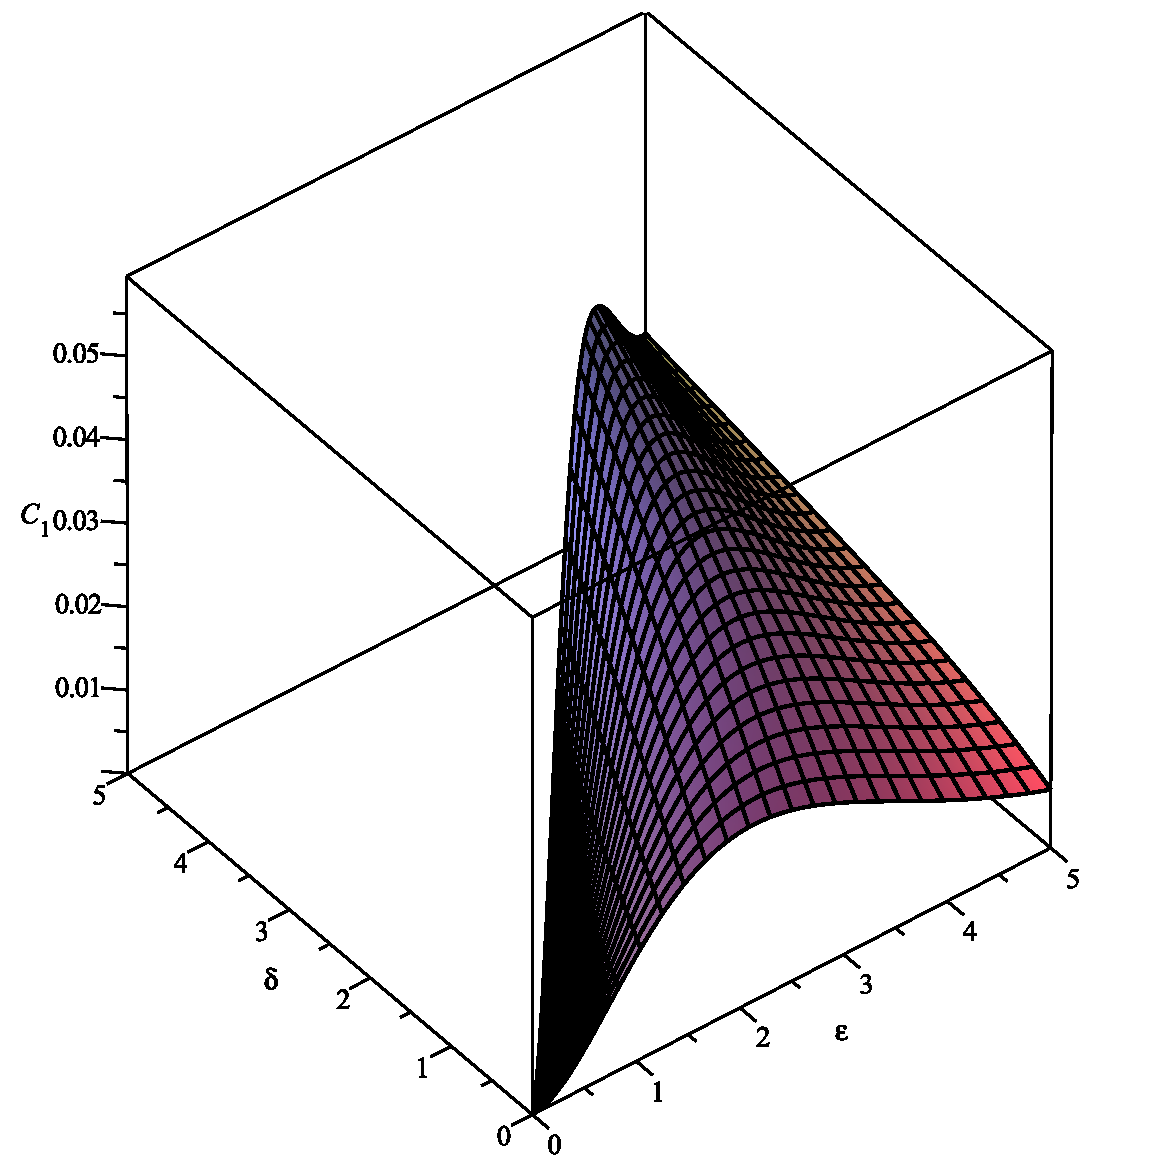
\includegraphics[height=0.44\textheight,keepaspectratio=true]{../src/plot/discreteSystems/C1InFunctionOfEpsilonAndDelta_2-eps-converted-to.pdf}
			\end{figure}
			\vspace{-25pt}
			\begin{figure}
				\centering
				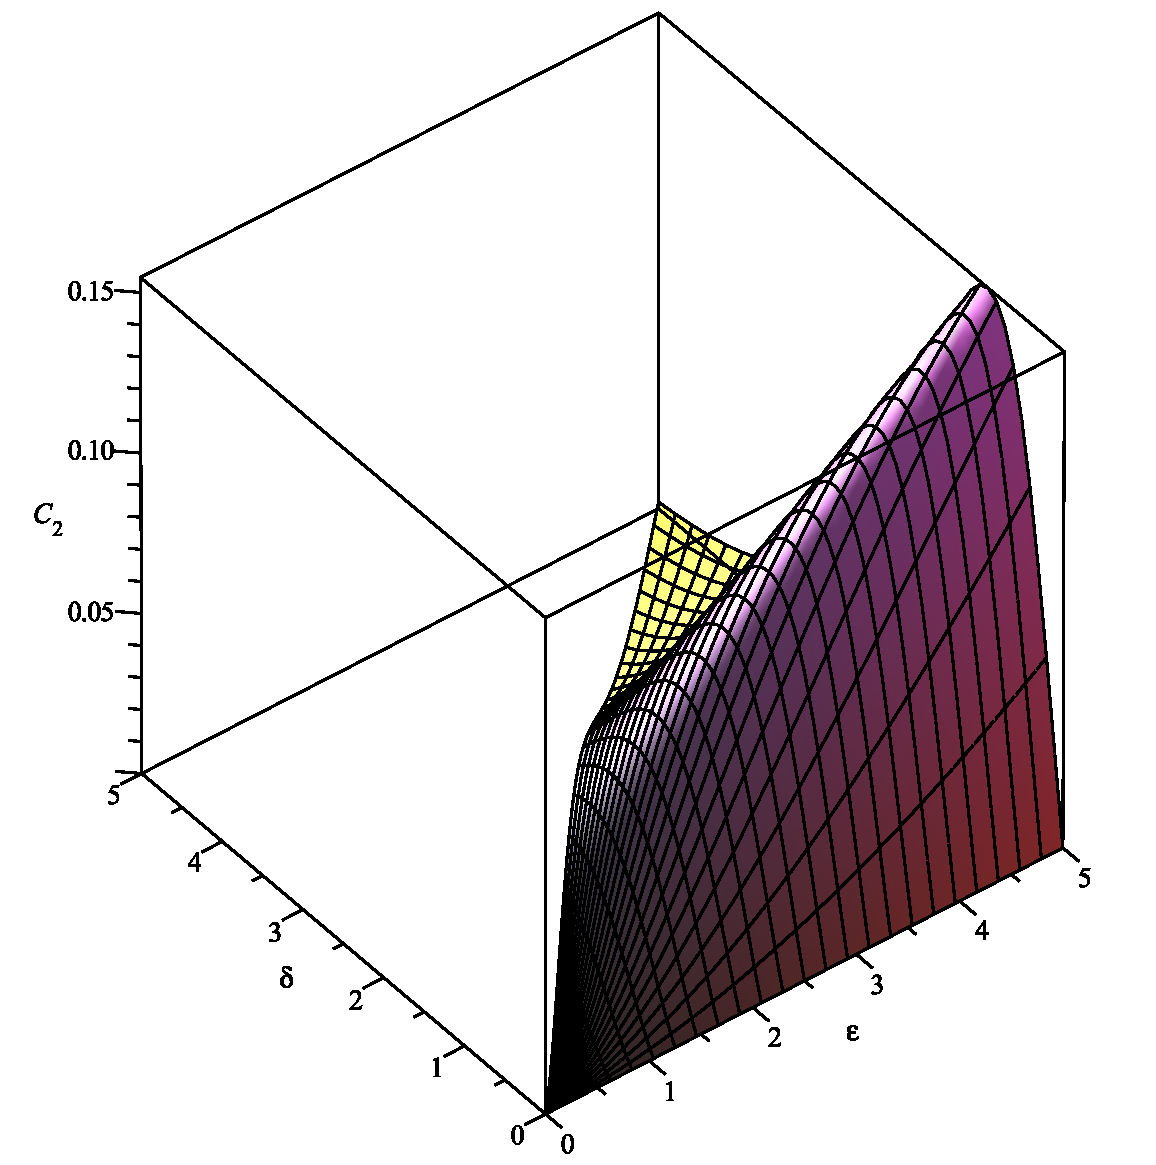
\includegraphics[height=0.44\textheight,keepaspectratio=true]{../src/plot/discreteSystems/C2InFunctionOfEpsilonAndDelta_2-eps-converted-to.pdf}
			\end{figure}
		\end{minipage}
	\end{tabular}

\end{frame}
